\documentclass[12pt, a4paper]{article}
\usepackage[utf8]{inputenc}
\usepackage{geometry}
\usepackage{titlesec}
\usepackage{enumitem}
\usepackage{hyperref}
\usepackage{graphicx}
\usepackage{fancyhdr}
\usepackage{amsmath}
\usepackage{amssymb}
\usepackage{float}
\usepackage{array}
\usepackage{booktabs}
\usepackage{longtable}
\usepackage[most]{tcolorbox}

% Page Geometry
\geometry{
	a4paper,
	total={170mm,257mm},
	left=20mm,
	top=25mm,
}

\setlength{\headheight}{15pt}

% Hyperlink Setup
\hypersetup{
	colorlinks=true,
	linkcolor=black,
	filecolor=magenta,      
	urlcolor=blue,
	citecolor=blue
}

% Header and Footer
\pagestyle{fancy}
\fancyhf{}
\rhead{Airline Reservation System - Phase 1}
\lhead{DBMS Project Report}
\cfoot{\thepage}

\begin{document}
	
	\begin{titlepage}
		\centering
		
		\IfFileExists{logo.png}{
			\begin{tabular}{c}
				
\includegraphics[width=0.25\textwidth]{logo.png} \\
				\vspace{0.1cm}
			\end{tabular}
		}{
			\framebox{\parbox{0.3\textwidth}{\centering \vspace{1cm} Logo Here \vspace{1cm}}}
		}
		
		\vspace{1.5cm}
		
		\hrule height 1pt
		\vspace{0.4cm}
		{\Large \textbf{\MakeUppercase{A DBMS Project On}}} \\
		\vspace{0.4cm}
		\hrule height 1pt
		
		\vspace{1cm}
		
		\begin{tcolorbox}[
			colback=black,      
			coltext=white,      
			colframe=black,     
			arc=0mm,            
			boxrule=0pt,        
			halign=center,      
			width=1\textwidth,  
			top=10mm, bottom=10mm 
			]
			\fontsize{20}{24}\selectfont \textbf{\MakeUppercase{Design and Implementation of an}} \\[0.5cm]
			\fontsize{20}{24}\selectfont \textbf{\MakeUppercase{Airline Reservation System}}
		\end{tcolorbox}
		
		\vspace{1cm}
		
		{\Large \textbf{\MakeUppercase{Submitted By}}}
		
		\vspace{0.5cm}
		
		\begin{tcolorbox}[
			colback=white, 
			colframe=black, 
			boxrule=1pt, 
			arc=0mm, 
			width=0.9\textwidth
			]
			\centering
			\renewcommand{\arraystretch}{1.5} 
			\begin{tabular}{r l}
				\textbf{Names:} & \textbf{Paranjoy Bordoloi  (24070122129)} \\
				& \textbf{Parmar Divyaansh  (24070122130)} \\
				& \textbf{Parth Sarathi Giri  (24070122132)} \\
				\textbf{Batch:} & 2024 - 2028 \\
				\textbf{Faculty:} & Prof. Jitendra Rajpurohit
			\end{tabular}
			
		\end{tcolorbox}
		\vspace{2cm}      
		{\text{{Department of Computer Science}}}\\
		{\text{{Symbiosis Institute of Technology, Pune}}}
		
	\end{titlepage}
	
	\tableofcontents
	\newpage
	
	\section{Introduction}
	
	\subsection{Contextual Overview of Aviation Data Management}
	The global aviation industry operates as a high-velocity network of logistics, customer service, and resource allocation, underpinned by complex information systems. At the core of this infrastructure lies the Airline Reservation System (ARS), a critical component of the broader Passenger Service System (PSS) \cite{ref1}. In the contemporary digital economy, an ARS is not merely a mechanism for booking tickets; it is a sophisticated database management challenge that requires the seamless integration of inventory control, fare tariffs, passenger records, and flight schedules \cite{ref2, ref3}. The efficacy of an airline's operations—and by extension, its profitability—is directly correlated with the robustness of its underlying database architecture.
	
	Historically, the management of airline reservations has evolved from labor-intensive manual processes to centralized mainframe environments, and finally to the distributed, web-enabled systems prevalent today \cite{ref4}. Early systems were standalone entities, isolated from travel agents and other carriers, leading to inefficiencies and data silos. The advent of Computerized Reservation Systems (CRS) and Global Distribution Systems (GDS) transformed the landscape, allowing for real-time connectivity between airlines and distribution channels \cite{ref5}. However, as airlines expand their routes and fleet sizes, legacy systems often struggle to maintain data consistency, concurrency, and scalability \cite{ref6}.
	
	This project report details the design and theoretical simulation of a next-generation Airline Reservation System database. Adhering to the Phase 1 rubrics of the Database Management System (DBMS) project guidelines \cite{ref7}, the report provides an exhaustive analysis of the problem domain, functional requirements, conceptual modeling, and logical schema design. By leveraging a Relational Database Management System (RDBMS), the proposed solution aims to eliminate the anomalies inherent in manual processing, ensure data integrity through rigorous normalization, and support the complex transactional needs of modern air travel \cite{ref8}.
	
	\subsection{Evolution from Manual to Digital Frameworks}
	To understand the necessity of a robust DBMS solution, one must examine the limitations of the manual and early digital predecessors. In pre-digital eras, or within the context of small regional carriers operating with minimal technology, reservations were tracked using physical cards or flat-file spreadsheets \cite{ref9}. This manual approach is fraught with peril: human error in data entry is rampant, retrieval of passenger history is sluggish, and the lack of real-time synchronization leads to significant operational risks such as overbooking or "lost" reservations \cite{ref10}.
	
	The transition to digital systems was driven by the need for speed and accuracy. Modern systems must handle thousands of concurrent transactions—users searching for flights, booking seats, and cancelling itineraries simultaneously—without compromising data validity \cite{ref11}. The shift from a flat-file approach to a relational model allows for the efficient storage of data across interconnected tables, reducing redundancy and improving retrieval times \cite{ref12}. Furthermore, the integration of web technologies has shifted the power dynamic, empowering passengers to manage their own bookings directly, a functional requirement that demands a user-friendly and highly responsive database backend \cite{ref13}.
	
	\subsection{Project Scope and Objectives}
	The primary objective of this project is to architect a database solution that addresses the systemic failures of legacy reservation methods. The scope of this "Phase 1" report encompasses the theoretical and logical design aspects of the system development life cycle.
	
	\noindent \textbf{Key Objectives:}
	\begin{itemize}
		\item \textbf{Systematize Requirements:} To translate vague business needs into concrete functional requirements and functional dependencies \cite{ref7}.
		\item \textbf{Conceptual Modeling:} To visualize the domain using Entity-Relationship (ER) and Enhanced Entity-Relationship (EER) diagrams, capturing the nuances of entity interactions such as the relationship between aircraft, flights, and routes \cite{ref14}.
		\item \textbf{Logical Design:} To derive a normalized relational schema that adheres to Codd’s rules, ensuring the database is free from update, insertion, and deletion anomalies \cite{ref7, ref15}.
		\item \textbf{Data Integrity:} To define constraints that preserve the accuracy of data, such as enforcing valid passport numbers and preventing overlapping flight schedules for the same aircraft \cite{ref16}.
	\end{itemize}
	
	The subsequent sections of this report will meticulously deconstruct these objectives, providing a blueprint for a system capable of managing the lifecycle of a flight reservation from initial query to final landing.
	
	\newpage
	\section{Problem Statement}
	
	\subsection{The Crisis of Legacy and Manual Systems}
	Despite the technological advancements in the broader industry, many airline sub-sectors and regional operators continue to rely on fragmented or poorly designed data management systems. The core problem addressed by this project is the inefficiency and operational risk introduced by these inadequate systems. A manual or flat-file based system is inherently incapable of handling the dynamic nature of modern aviation \cite{ref17}.
	
	\noindent \textbf{Operational Inefficiencies:} \\
	In a manual system, the process of booking a ticket involves a human operator physically checking a ledger or a standalone spreadsheet for seat availability. This introduces a critical latency; by the time the operator confirms availability, another agent might have already sold the seat \cite{ref10}. This lack of concurrency control is a primary cause of double-booking, which results in revenue loss and severe customer dissatisfaction. Furthermore, manual systems make the retrieval of passenger records—essential for security checks and customer service—an arduous task involving physical searches through files \cite{ref11}.
	
	\noindent \textbf{Data Redundancy and Inconsistency:} \\
	Without a centralized RDBMS, data is often duplicated across different departments. The flight operations team might have one record of a flight's schedule, while the ticketing office has another. If a flight is delayed, this information often fails to propagate to the ticketing system in real-time, leaving passengers uninformed \cite{ref18}. This inconsistency is a classic symptom of un-normalized data storage, where the same fact (e.g., flight departure time) is stored in multiple locations, leading to update anomalies.
	
	\subsection{Specific Operational Pain Points}
	The following specific challenges have been identified through domain analysis and serve as the drivers for the proposed system design:
	
	\begin{enumerate}
		\item \textbf{Inability to Select Seats:} A major deficiency in older systems is the lack of a visual seat map. Passengers are often assigned seats arbitrarily at the check-in counter, disregarding preferences for window or aisle seats \cite{ref10}. This manual assignment slows down the check-in process and reduces passenger satisfaction.
		\item \textbf{Notification Failures:} Legacy systems lack automated triggers. When a flight is cancelled or delayed due to weather, there is no automatic mechanism to query the \texttt{Passenger} database and dispatch notifications via SMS or email \cite{ref13, ref18}.
		\item \textbf{Complex Fare Calculation Errors:} Manual calculation of fares, which involves base rates, taxes, fuel surcharges, and dynamic class-based pricing, is prone to human arithmetic error. This can lead to financial leakage for the airline or overcharging of customers \cite{ref2}.
		\item \textbf{Lack of Historical Insight:} Without a structured query language (SQL) capability, generating reports on route profitability, passenger demographics, or seasonal trends is virtually impossible \cite{ref19}. Management lacks the data-driven insights necessary for strategic planning.
		\item \textbf{Security and Access Control:} Flat-file systems do not offer granular access control. A ticketing agent should not have the same database privileges as a system administrator. The lack of role-based security in legacy systems poses a significant threat to data privacy \cite{ref20}.
	\end{enumerate}
	
	\subsection{The Imperative for a Relational Solution}
	The solution to these multifaceted problems lies in the implementation of a centralized Airline Reservation System built on a Relational Database Management System (RDBMS). An RDBMS solves the concurrency issue through transaction locking mechanisms (ACID properties), ensures data consistency through referential integrity constraints, and eliminates redundancy through normalization \cite{ref12}. The proposed system will replace the fragmented manual processes with a unified platform where a change in one module (e.g., Flight Scheduling) instantly reflects in all others (e.g., Booking and Notifications).
	
	\newpage
	\section{System Architecture and Modules}
	
	\begin{figure}[H]
		\centering
		\IfFileExists{new.png}{
			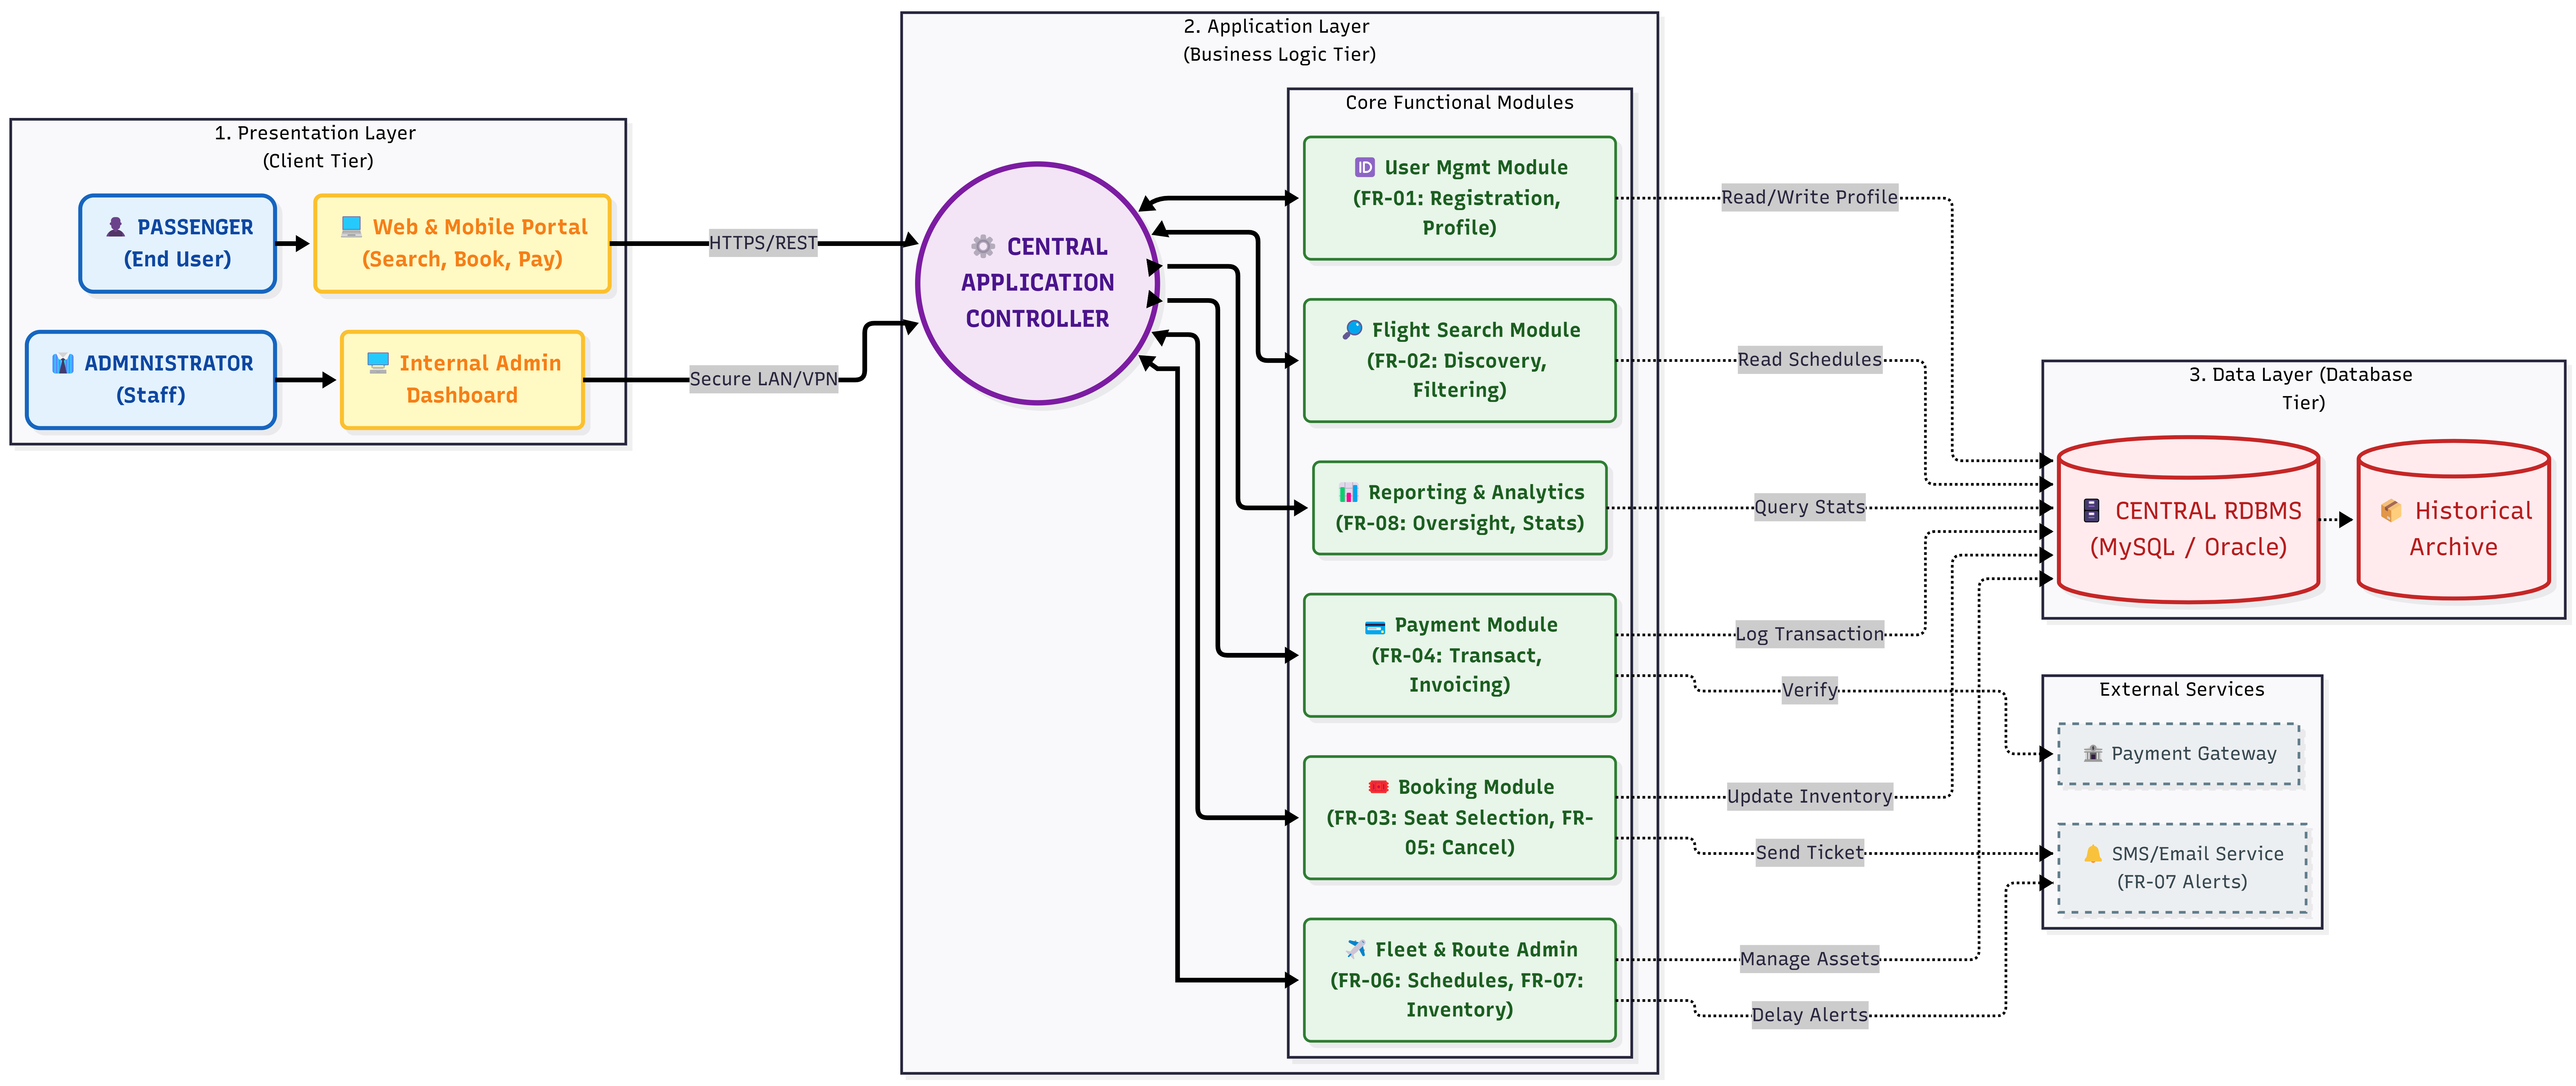
\includegraphics[width=1.0\textwidth]{new.png}
		}{
			\framebox{\parbox{0.8\textwidth}{\centering
					\vspace{3cm}
					\textbf{Image not found: new.png} \\
					\small Please ensure the file "new.png" is in the same directory.
					\vspace{3cm}
			}}
		}
		\caption{Three-Tier Architecture of the Airline Reservation System illustrating the interaction between Client, Application, and Data layers.}
		\label{fig:Arch_diagram}
	\end{figure}
	
	\subsection{Architectural Framework}
	The proposed Airline Reservation System utilizes a multi-tier client-server architecture, designed to ensure scalability, security, and ease of maintenance \cite{ref21, ref22}.
	
	\begin{itemize}
		\item \textbf{Presentation Layer (Client Tier):} This layer provides the interface for end-users (passengers) and internal users (administrators, staff). For passengers, this is a web-based portal accessible via browsers, facilitating flight search and booking \cite{ref23}. For staff, a secure intranet portal provides access to administrative functions.
		\item \textbf{Application Layer (Business Logic Tier):} This middle tier hosts the core application logic. It processes requests from the client, enforces business rules (e.g., "a passenger cannot book a seat on a departed flight"), and manages sessions. It serves as the intermediary, preventing direct user access to the database \cite{ref24}.
		\item \textbf{Data Layer (Database Tier):} The foundation of the system is the RDBMS (e.g., MySQL or Oracle). This layer stores all persistent data, including flight inventories, passenger profiles, and transaction logs. It is responsible for data integrity, backup, and query execution \cite{ref25}.
	\end{itemize}
	
	\subsection{Functional Module Breakdown}
	The system is decomposed into distinct functional modules, each addressing specific business requirements identified in the problem statement.
	
	\subsubsection{User Registration and Management Module}
	This module handles the lifecycle of user identities within the system. It distinguishes between distinct user roles: Passengers and Administrators \cite{ref26}.
	\begin{itemize}
		\item \textbf{Functionality:} Allows new customers to register by providing personal details (Name, Address, Passport Info) \cite{ref2}. It manages secure login authentication via password hashing and session management \cite{ref26}.
		\item \textbf{Data Interaction:} Interacts primarily with the \texttt{Passenger} and \texttt{Login\_Credentials} tables.
	\end{itemize}
	
	\subsubsection{Flight Search and Inquiry Module}
	This is the primary interface for customer interaction. It allows users to query the database for flight availability based on specific criteria.
	\begin{itemize}
		\item \textbf{Functionality:} Enables searching by Origin, Destination, Date, and Class (Economy, Business). It retrieves flight schedules, durations, and pricing \cite{ref9, ref26}.
		\item \textbf{Data Interaction:} Executes complex \texttt{SELECT} queries with \texttt{JOIN} operations across \texttt{Flight}, \texttt{Route}, \texttt{Airport}, and \texttt{Fare} tables.
	\end{itemize}
	
	\subsubsection{Booking and Reservation Module}
	This core module manages the transactional aspect of selling seats. It is the most complex module as it involves concurrency control and inventory management \cite{ref2}.
	\begin{itemize}
		\item \textbf{Functionality:} Facilitates seat selection (visual map), passenger detail entry, and provisional booking creation. It checks the \texttt{AvailableSeats} attribute to prevent overbooking \cite{ref27}.
		\item \textbf{Data Interaction:} Performs \texttt{INSERT} operations into the \texttt{Booking} and \texttt{Ticket} tables and \texttt{UPDATE} operations on the \texttt{Flight} inventory.
	\end{itemize}
	
	\subsubsection{Payment and Transaction Module}
	Responsible for the financial settlement of bookings.
	\begin{itemize}
		\item \textbf{Functionality:} Processes payments via integrated gateways, generates invoices, and updates the payment status of a booking from 'Pending' to 'Confirmed' \cite{ref16, ref28}.
		\item \textbf{Data Interaction:} Manages the \texttt{Payment} and \texttt{Transaction} tables, ensuring a 1:1 link with the \texttt{Booking} table \cite{ref29}.
	\end{itemize}
	
	\subsubsection{Administrator and Flight Management Module}
	A restricted-access module for airline operations staff to manage the supply side of the system.
	\begin{itemize}
		\item \textbf{Functionality:} Allows admins to Add, Modify, or Delete flight schedules and routes \cite{ref26}. It also includes inventory control—assigning specific aircraft to routes based on capacity needs \cite{ref30}.
		\item \textbf{Data Interaction:} Direct manipulation of \texttt{Flight}, \texttt{Aircraft}, \texttt{Route}, and \texttt{Employee} tables.
	\end{itemize}
	
	\subsubsection{Cancellation and Notification Module}
	Addresses the post-booking lifecycle and exception handling.
	\begin{itemize}
		\item \textbf{Functionality:} Allows passengers to cancel bookings, triggering a refund calculation and releasing the seat back to inventory \cite{ref2}. It also monitors flight status changes (delays) and triggers notifications \cite{ref10, ref31}.
		\item \textbf{Data Interaction:} Updates \texttt{Booking} status and \texttt{Flight} seat counts.
	\end{itemize}
	
	\newpage
	\section{Functional Requirements}
	
	The functional requirements define the specific behaviors the system must exhibit to meet the business needs. These are categorized by the user roles interacting with the system.
	
	\subsection{Passenger Functional Requirements}
	
	\textbf{FR-01: Registration and Profile Management}
	\begin{itemize}
		\item The system shall allow unregistered users to create an account by providing a valid email address, password, full name, and phone number \cite{ref26}.
		\item The system shall allow registered users to view and update their profile information, including passport details and frequent flyer numbers \cite{ref32}.
		\item The system must validate that the password meets security complexity standards (e.g., minimum length, special characters) \cite{ref2}.
	\end{itemize}
	
	\textbf{FR-02: Flight Search and Discovery}
	\begin{itemize}
		\item The system shall provide a search interface where users enter Origin City, Destination City, and Travel Date \cite{ref9, ref32}.
		\item The system shall display a list of available flights that match the criteria, showing Flight Number, Departure/Arrival Times, Duration, and Price \cite{ref33}.
		\item The system shall allow users to sort search results by Price (Low to High) or Duration (Shortest to Longest) \cite{ref26}.
		\item The system shall handle queries where no direct flight exists by suggesting connecting flights (if implemented) or displaying a "No Flights Available" message \cite{ref9}.
	\end{itemize}
	
	\textbf{FR-03: Seat Selection and Booking}
	\begin{itemize}
		\item The system shall display a graphical seat map for the selected flight, indicating occupied and available seats \cite{ref32}.
		\item The system shall allow the user to select a seat based on class (Economy, Business) \cite{ref10}.
		\item The system shall lock the selected seat for a predefined duration (e.g., 10 minutes) during the payment process to prevent double-booking \cite{ref29}.
		\item The system shall collect passenger details (Name, Age, Gender) for all travelers in the booking \cite{ref9}.
	\end{itemize}
	
	\textbf{FR-04: Payment and Ticketing}
	\begin{itemize}
		\item The system shall calculate the total fare, including base fare, taxes, and service charges \cite{ref9}.
		\item The system shall accept payment information and process the transaction securely \cite{ref16}.
		\item Upon successful payment, the system shall generate a unique Booking Reference Number (PNR) and a digital ticket/itinerary \cite{ref32}.
	\end{itemize}
	
	\textbf{FR-05: Booking Management and Cancellation}
	\begin{itemize}
		\item The system shall allow users to retrieve their booking using the PNR and Last Name \cite{ref13}.
		\item The system shall allow users to cancel a booking. The system must calculate the refund amount based on the cancellation policy and the time remaining before departure \cite{ref26}.
		\item The system shall allow users to print their boarding pass or ticket \cite{ref10}.
	\end{itemize}
	
	\subsection{Administrator Functional Requirements}
	
	\textbf{FR-06: Flight and Route Administration}
	\begin{itemize}
		\item The system shall allow administrators to create new flight schedules, specifying the aircraft, route, and timing \cite{ref26}.
		\item The system shall allow administrators to modify existing flight details (e.g., change departure time) or cancel flights entirely \cite{ref20}.
		\item The system shall allow the definition of new Routes (Origin and Destination pairs) \cite{ref14}.
	\end{itemize}
	
	\textbf{FR-07: Inventory and Fleet Management}
	\begin{itemize}
		\item The system shall allow administrators to add new aircraft to the fleet, specifying the Model, Manufacturer, and Capacity \cite{ref14}.
		\item The system shall allow the assignment of crew members (Pilots, Cabin Crew) to specific flights \cite{ref20}.
	\end{itemize}
	
	\textbf{FR-08: Reporting and Oversight}
	\begin{itemize}
		\item The system shall provide a dashboard for administrators to view booking statistics, revenue reports, and flight occupancy rates \cite{ref26}.
		\item The system shall allow administrators to view the passenger manifest for any flight \cite{ref30}.
	\end{itemize}
	
	\subsection{System/Non-Functional Requirements Impacting Database Design}
	
	\textbf{FR-09: Data Integrity and Validation}
	\begin{itemize}
		\item The system shall ensure that a flight cannot be scheduled if the assigned aircraft is already in use during that time block (Integrity Constraint) \cite{ref16}.
		\item The system shall ensure that the number of bookings for a flight does not exceed the aircraft's capacity \cite{ref16}.
	\end{itemize}
	
	\textbf{FR-10: Scalability and Performance}
	\begin{itemize}
		\item The database must support indexing on high-frequency search columns (e.g., \texttt{DepartureDate}, \texttt{Origin}, \texttt{Destination}) to ensure search results are returned in under 5 seconds \cite{ref34}.
	\end{itemize}
	
	\newpage
	\section{Entities, Attributes, and Relationships}
	
	The Conceptual Design phase involves identifying the core entities that make up the airline domain and defining their attributes. This serves as the foundation for the ER diagram.
	
	\subsection{Entity Identification and Attribute Definition}
	
	Based on the research analysis \cite{ref16, ref35, ref36, ref37}, the following entities have been identified.
	
	\begin{enumerate}
		\item \textbf{Passenger (Traveler)}
		\begin{itemize}
			\item Represents the individual who utilizes the airline service.
			\item \textbf{Attributes:}
			\begin{itemize}
				\item \texttt{PassengerID} (Primary Key): A unique integer identifier for internal referencing.
				\item \texttt{FirstName}: String.
				\item \texttt{LastName}: String.
				\item \texttt{PassportNumber}: String (Alphanumeric). Essential for international travel and identity verification. Must be unique.
				\item \texttt{Email}: String. Used for sending tickets and notifications.
				\item \texttt{Phone}: String. Contact number for SMS alerts.
				\item \texttt{Address}: String. Billing or physical address.
				\item \texttt{Age}: Integer. Used to categorize passengers (Adult, Child, Infant) for fare calculation.
			\end{itemize}
		\end{itemize}
		
		\item \textbf{Flight (Scheduled Service)}
		\begin{itemize}
			\item Represents a specific journey scheduled for a specific date and time.
			\item \textbf{Attributes:}
			\begin{itemize}
				\item \texttt{FlightID} (Primary Key): Unique identifier.
				\item \texttt{FlightNumber}: String (e.g., "AI202"). Note that flight numbers are reused; \texttt{FlightID} distinguishes the specific instance on a specific date.
				\item \texttt{DepartureTime}: DateTime.
				\item \texttt{ArrivalTime}: DateTime.
				\item \texttt{Status}: String/Enum (Scheduled, Delayed, Cancelled, Departed).
				\item \texttt{AvailableSeats}: Integer. Tracks real-time inventory.
			\end{itemize}
		\end{itemize}
		
		\item \textbf{Airport (Location)}
		\begin{itemize}
			\item Represents the physical infrastructure where flights originate and terminate.
			\item \textbf{Attributes:}
			\begin{itemize}
				\item \texttt{AirportCode} (Primary Key): String (3 chars). Standard IATA code (e.g., LHR, DXB).
				\item \texttt{Name}: String. Full name of the airport.
				\item \texttt{City}: String.
				\item \texttt{Country}: String.
				\item \texttt{Timezone}: String. Crucial for calculating duration correctly across zones.
			\end{itemize}
		\end{itemize}
		
		\item \textbf{Route (Path)}
		\begin{itemize}
			\item Represents the logical connection between two airports.
			\item \textbf{Attributes:}
			\begin{itemize}
				\item \texttt{RouteID} (Primary Key): Unique identifier.
				\item \texttt{Distance}: Integer. Used for fuel and fare calculations.
				\item \texttt{EstimatedDuration}: Time. Standard flight time for this path.
			\end{itemize}
		\end{itemize}
		
		\item \textbf{Aircraft (Physical Asset)}
		\begin{itemize}
			\item Represents the specific plane assigned to a flight.
			\item \textbf{Attributes:}
			\begin{itemize}
				\item \texttt{AircraftID} (Primary Key): Unique identifier.
				\item \texttt{RegistrationNumber}: String. Tail number (e.g., N12345).
				\item \texttt{Model}: String (e.g., "Boeing 737").
				\item \texttt{Manufacturer}: String.
				\item \texttt{TotalCapacity}: Integer.
				\item \texttt{BusinessSeats}: Integer.
				\item \texttt{EconomySeats}: Integer.
			\end{itemize}
		\end{itemize}
		
		\item \textbf{Booking (Reservation)}
		\begin{itemize}
			\item Represents the contract between the passenger and the airline.
			\item \textbf{Attributes:}
			\begin{itemize}
				\item \texttt{BookingID} (Primary Key): Unique PNR.
				\item \texttt{BookingDate}: DateTime.
				\item \texttt{TravelClass}: String (Economy, Business).
				\item \texttt{SeatNumber}: String (e.g., "12A").
				\item \texttt{Status}: String (Confirmed, Cancelled, Pending).
				\item \texttt{TotalAmount}: Decimal.
			\end{itemize}
		\end{itemize}
		
		\item \textbf{Payment (Financial Transaction)}
		\begin{itemize}
			\item Represents the exchange of funds for the booking.
			\item \textbf{Attributes:}
			\begin{itemize}
				\item \texttt{PaymentID} (Primary Key): Unique identifier.
				\item \texttt{Amount}: Decimal.
				\item \texttt{PaymentMethod}: String (Credit Card, PayPal).
				\item \texttt{TransactionDate}: DateTime.
				\item \texttt{TransactionReference}: String. Gateway confirmation code.
			\end{itemize}
		\end{itemize}
		
		\item \textbf{Employee (Staff)}
		\begin{itemize}
			\item Represents airline personnel involved in operations.
			\item \textbf{Attributes:}
			\begin{itemize}
				\item \texttt{EmployeeID} (Primary Key).
				\item \texttt{Name}: String.
				\item \texttt{Role}: String (Pilot, Crew, Admin).
				\item \texttt{DateHired}: Date.
			\end{itemize}
		\end{itemize}
	\end{enumerate}
	
	\subsection{Relationship Analysis and Cardinalities}
	
	The interaction between these entities defines the business logic of the system \cite{ref14, ref38}.
	
	\begin{itemize}
		\item \textbf{Passenger - Booking:}
		\begin{itemize}
			\item \textbf{Relationship:} A Passenger \textit{Makes} a Booking.
			\item \textbf{Cardinality:} One-to-Many (1:N). A passenger can make multiple bookings over time. A specific booking record is associated with one primary passenger.
		\end{itemize}
		\item \textbf{Flight - Booking:}
		\begin{itemize}
			\item \textbf{Relationship:} A Booking \textit{Is\_For} a Flight.
			\item \textbf{Cardinality:} One-to-Many (1:N). One flight holds many bookings. A single booking (ticket) is for one specific flight leg.
		\end{itemize}
		\item \textbf{Flight - Aircraft:}
		\begin{itemize}
			\item \textbf{Relationship:} A Flight \textit{Uses} an Aircraft.
			\item \textbf{Cardinality:} Many-to-One (N:1). An aircraft flies many flights over its lifetime. A specific flight instance uses exactly one aircraft.
		\end{itemize}
		\item \textbf{Flight - Route:}
		\begin{itemize}
			\item \textbf{Relationship:} A Flight \textit{Follows} a Route.
			\item \textbf{Cardinality:} Many-to-One (N:1). Multiple flight instances (e.g., the daily 9 AM flight) follow the same defined route.
		\end{itemize}
		\item \textbf{Route - Airport:}
		\begin{itemize}
			\item \textbf{Relationship:} A Route \textit{Connects} Airports.
			\item \textbf{Cardinality:} Binary relationship linking an Origin Airport and a Destination Airport.
		\end{itemize}
		\item \textbf{Booking - Payment:}
		\begin{itemize}
			\item \textbf{Relationship:} A Booking \textit{Generates} a Payment.
			\item \textbf{Cardinality:} One-to-One (1:1). For this system design, we assume one booking has one associated payment transaction \cite{ref29}.
		\end{itemize}
		\item \textbf{Employee - Flight:}
		\begin{itemize}
			\item \textbf{Relationship:} Employees \textit{Operate} a Flight.
			\item \textbf{Cardinality:} Many-to-Many (M:N). A flight requires a crew (multiple employees). An employee works on multiple flights. This requires an associative entity \texttt{Crew\_Assignment} \cite{ref39}.
		\end{itemize}
	\end{itemize}
	
	\subsection{Relationship Analysis Table}
	
	The interaction between these entities defines the business logic of the system. The cardinalities and relationships are summarized below.
	
	\begin{table}[H]
		\centering
		\renewcommand{\arraystretch}{1.5}
		\begin{tabular}{|l|p{3cm}|l|l|p{4cm}|}
			\hline
			\textbf{Entity A} & \textbf{Relationship} & \textbf{Entity B} & \textbf{Cardinality} & \textbf{Description} \\
			\hline
			Passenger & Makes & Booking & 1:N & A passenger can make multiple bookings; a booking belongs to one passenger. \\
			\hline
			Booking & Is\_For & Flight & N:1 & Multiple bookings exist for a single flight; a ticket is for one specific flight. \\
			\hline
			Flight & Uses & Aircraft & N:1 & An aircraft is reused for many flights; a scheduled flight uses one aircraft. \\
			\hline
			Flight & Follows & Route & N:1 & Many flights follow the same path; a specific flight schedule follows one route. \\
			\hline
			Route & Connects & Airport & M:N & A route connects two airports (Origin and Destination). \\
			\hline
			Booking & Generates & Payment & 1:1 & Each confirmed booking has exactly one payment record. \\
			\hline
			Employee & Operates & Flight & M:N & Multiple crew operate a flight; employees work on multiple flights. \\
			\hline
		\end{tabular}
		\caption{Relationship Analysis and Cardinalities}
		\label{tab:relationship_matrix}
	\end{table}
	
	\newpage
	\section{Conceptual Design: ER and EER Diagrams}
	
	The Entity-Relationship (ER) model provides a graphical representation of the logical structure of the database. This section describes the components and the advanced modeling concepts used.
	
	\subsection{ER Diagram Components}
	
	The ER diagram for the Airline Reservation System is constructed using standard Crow's Foot notation concepts.
	
	\begin{itemize}
		\item \textbf{Strong Entities:} \texttt{Passenger}, \texttt{Flight}, \texttt{Airport}, \texttt{Aircraft}, \texttt{Airline}, \texttt{Route}. These entities have their own primary keys and exist independently.
		\item \textbf{Weak Entities:} \texttt{Seat} can be modeled as a weak entity dependent on \texttt{Aircraft} (identified by \texttt{SeatNumber} + \texttt{AircraftID}), though often it is simplified as an attribute in smaller designs. In this comprehensive report, \texttt{Ticket} is often considered a weak entity dependent on \texttt{Booking} if modeled separately \cite{ref40}.
		\item \textbf{Associative Entities:} \texttt{Crew\_Assignment} resolves the many-to-many relationship between \texttt{Employee} and \texttt{Flight}. It contains attributes like \texttt{Role\_In\_Flight} (e.g., Pilot, Co-Pilot, Head Steward) \cite{ref41}.
	\end{itemize}
	
	\textbf{Diagram Narrative:}
	The central hub is the \texttt{Flight} entity. It has outgoing relationships to \texttt{Airport} (Origin and Destination), \texttt{Aircraft} (the physical plane), and \texttt{Route} (the path). The \texttt{Booking} entity acts as the transactional link, connecting \texttt{Passenger} to \texttt{Flight}. \texttt{Payment} is an appendage to \texttt{Booking}, strictly 1:1.
	
	% ER DIAGRAM IMAGE - FORCED PLACEMENT [H]
	\begin{figure}[H]
		\centering
		\IfFileExists{er_diagram.png}{
			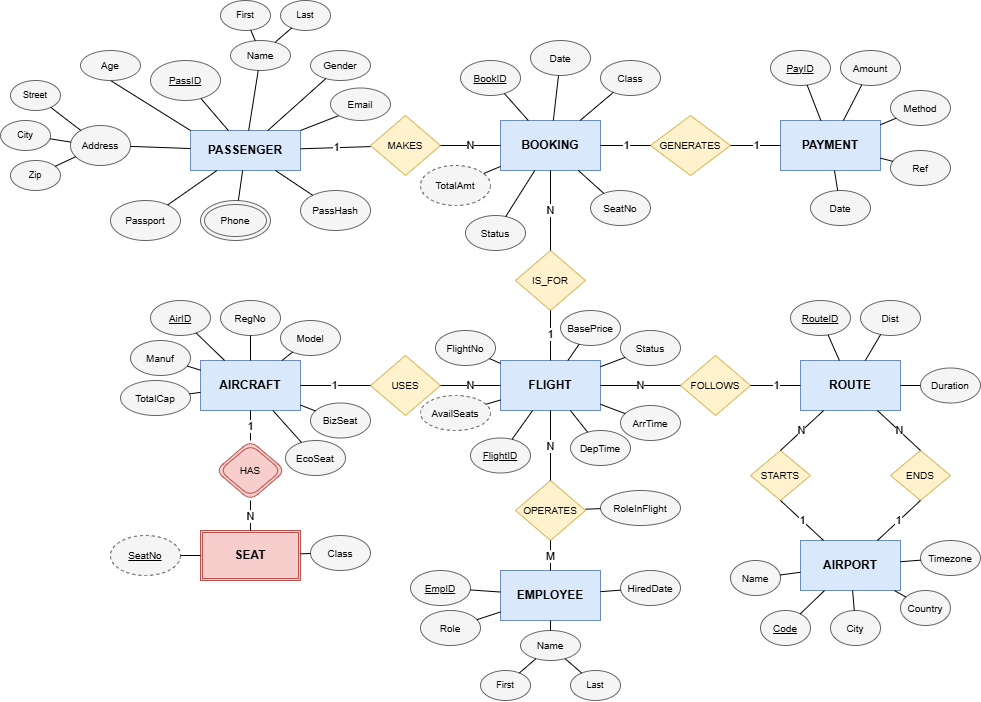
\includegraphics[width=1.0\textwidth]{er_diagram.png}
		}{
			\framebox{\parbox{0.8\textwidth}{\centering
					\vspace{3cm}
					\textbf{Image not found: er\_diagram.png} \\
					\small Please ensure the file "er\_diagram.png" is in the same directory.
					\vspace{3cm}
			}}
		}
		\caption{Entity-Relationship (ER) Diagram for Airline Reservation System}
		\label{fig:er_diagram}
	\end{figure}
	
	\subsection{Enhanced Entity-Relationship (EER) Modeling}
	
	To capture the complexity of the domain effectively, Enhanced ER concepts such as \textbf{Generalization} (Superclass/Subclass) and \textbf{Specialization} are employed \cite{ref42, ref43}.
	
	% EER DIAGRAM IMAGE - FORCED PLACEMENT [H]
	\begin{figure}[H]
		\centering
		\IfFileExists{eer_diagram2.png}{
			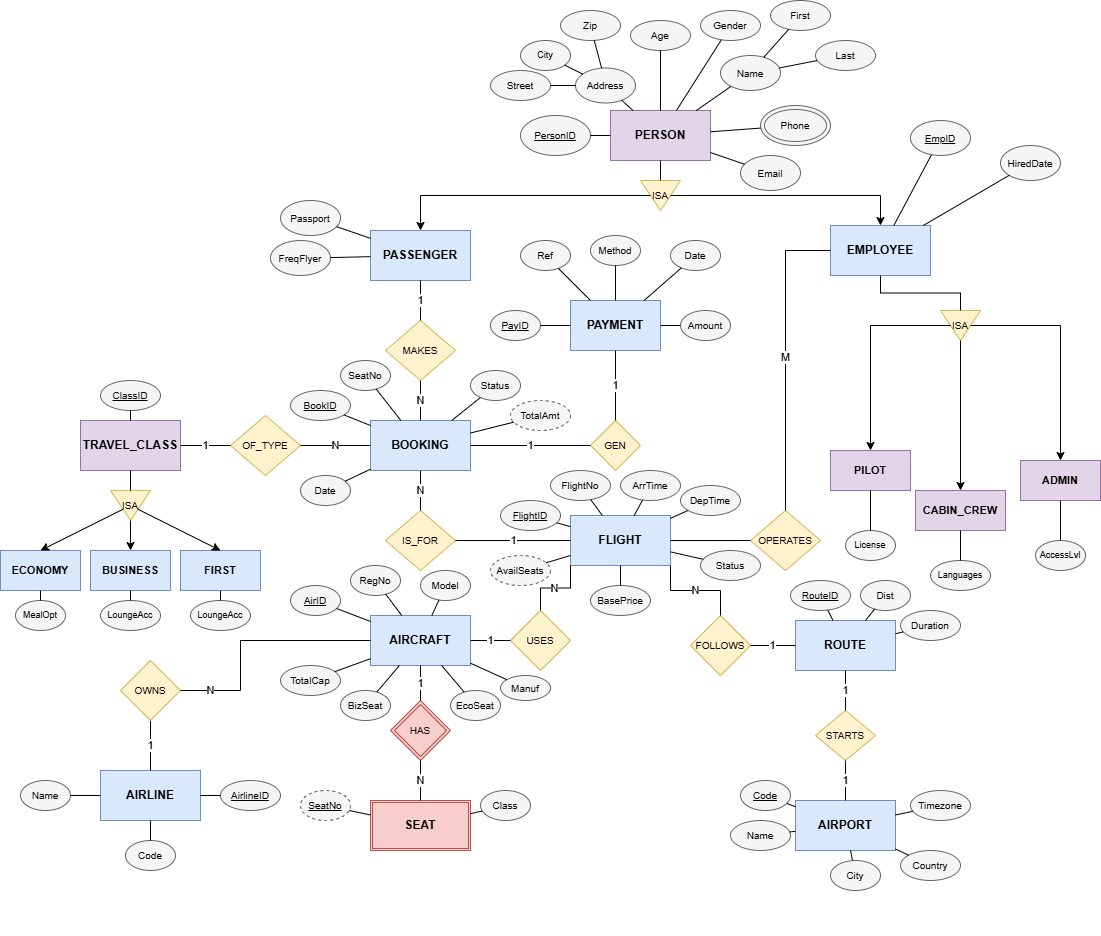
\includegraphics[width=1.0\textwidth]{eer_diagram2.png}
		}{
			\framebox{\parbox{0.8\textwidth}{\centering
					\vspace{3cm}
					\textbf{Image not found: eer\_diagram.png} \\
					\small Please ensure the file "eer\_diagram.png" is in the same directory.
					\vspace{3cm}
			}}
		}
		\caption{Enhanced Entity-Relationship (EER) Diagram}
		\label{fig:eer_diagram}
	\end{figure}
	
	\subsubsection{Person Generalization}
	There is a significant overlap in attributes between \texttt{Passenger} and \texttt{Employee} (Name, Address, Contact Info).
	\begin{itemize}
		\item \textbf{Superclass:} \texttt{Person}
		\begin{itemize}
			\item Attributes: \texttt{PersonID}, \texttt{Name}, \texttt{Address}, \texttt{PhoneNumber}, \texttt{Email}.
		\end{itemize}
		\item \textbf{Subclasses:}
		\begin{itemize}
			\item \texttt{Passenger}: Adds \texttt{PassportNumber}, \texttt{FrequentFlyerMiles}.
			\item \texttt{Employee}: Adds \texttt{EmployeeID}, \texttt{Salary}, \texttt{Department}.
		\end{itemize}
		\item \textbf{Constraint:} This is an \textbf{Overlapping} specialization (a person could theoretically be both an employee and a passenger) and \textbf{Partial} participation (a person might exist in the system as a contact reference without being either active role) \cite{ref41}.
	\end{itemize}
	
	\subsubsection{Employee Specialization}
	Within the \texttt{Employee} entity, distinct roles require different data points \cite{ref39}.
	\begin{itemize}
		\item \textbf{Superclass:} \texttt{Employee}
		\item \textbf{Subclasses:}
		\begin{itemize}
			\item \texttt{Pilot}: Attributes include \texttt{LicenseNumber}, \texttt{FlightHoursLog}, \texttt{MedicalCertExpiry}.
			\item \texttt{CabinCrew}: Attributes include \texttt{LanguageSkills}.
			\item \texttt{AdminStaff}: Attributes include \texttt{AccessLevel}, \texttt{SystemPrivileges}.
		\end{itemize}
		\item \textbf{Constraint:} \textbf{Disjoint} (an employee typically performs one primary role at a time) and \textbf{Total} participation (every employee must be assigned a role).
	\end{itemize}
	
	\subsubsection{Travel Class Specialization}
	\begin{itemize}
		\item \textbf{Superclass:} \texttt{TravelClass}
		\item \textbf{Subclasses:} \texttt{Economy}, \texttt{Business}, \texttt{First}.
		\item This allows the system to store class-specific attributes, such as \texttt{LoungeAccess} (Boolean) for Business/First, or \texttt{MealSelection} options \cite{ref44}.
	\end{itemize}
	
	\newpage
	\section{Relational Schema}
	
	The conceptual ER/EER model is transformed into a logical Relational Schema. This involves mapping entities to tables, attributes to columns, and relationships to foreign keys.
	
	\subsection{Table Definitions}
	
	\begin{table}[H]
		\centering
		\caption{Table: Airport}
		\begin{tabular}{|l|l|l|p{5cm}|}
			\hline
			\textbf{Attribute} & \textbf{Data Type} & \textbf{Constraints} & \textbf{Description} \\
			\hline
			AirportCode & VARCHAR(3) & PK & Standard IATA code (e.g., LHR). \\
			\hline
			Name & VARCHAR(100) & NOT NULL & Full name of the airport. \\
			\hline
			City & VARCHAR(50) & NOT NULL & Location city. \\
			\hline
			Country & VARCHAR(50) & NOT NULL & Location country. \\
			\hline
		\end{tabular}
	\end{table}
	\noindent \textbf{Schema:} \texttt{Airport (\underline{AirportCode}, Name, City, Country)}
	
	\begin{table}[H]
		\centering
		\caption{Table: Airline}
		\begin{tabular}{|l|l|l|p{5cm}|}
			\hline
			\textbf{Attribute} & \textbf{Data Type} & \textbf{Constraints} & \textbf{Description} \\
			\hline
			AirlineID & INT & PK & Unique identifier. \\
			\hline
			Name & VARCHAR(100) & NOT NULL & Name of the airline. \\
			\hline
			Code & VARCHAR(3) & Unique & ICAO/IATA Airline code. \\
			\hline
		\end{tabular}
	\end{table}
	\noindent \textbf{Schema:} \texttt{Airline (\underline{AirlineID}, Name, Code)}
	
	\begin{table}[H]
		\centering
		\caption{Table: Aircraft}
		\begin{tabular}{|l|l|l|p{5cm}|}
			\hline
			\textbf{Attribute} & \textbf{Data Type} & \textbf{Constraints} & \textbf{Description} \\
			\hline
			AircraftID & INT & PK & Unique identifier. \\
			\hline
			RegistrationNumber & VARCHAR(20) & Unique & Tail number (e.g., N12345). \\
			\hline
			Model & VARCHAR(50) & NOT NULL & Aircraft model. \\
			\hline
			Capacity & INT & NOT NULL & Total seating capacity. \\
			\hline
			AirlineID & INT & FK & References Airline. \\
			\hline
		\end{tabular}
	\end{table}
	\noindent \textbf{Schema:} \texttt{Aircraft (\underline{AircraftID}, RegistrationNumber, Model, Capacity, \textit{AirlineID})}
	
	\begin{table}[H]
		\centering
		\caption{Table: Route}
		\begin{tabular}{|l|l|l|p{5cm}|}
			\hline
			\textbf{Attribute} & \textbf{Data Type} & \textbf{Constraints} & \textbf{Description} \\
			\hline
			RouteID & INT & PK & Unique identifier. \\
			\hline
			OriginCode & VARCHAR(3) & FK & References Airport (Origin). \\
			\hline
			DestCode & VARCHAR(3) & FK & References Airport (Dest). \\
			\hline
			Distance & INT & & Distance in Km/Miles. \\
			\hline
		\end{tabular}
	\end{table}
	\noindent \textbf{Schema:} \texttt{Route (\underline{RouteID}, \textit{OriginCode}, \textit{DestCode}, Distance)}
	
	\begin{table}[H]
		\centering
		\caption{Table: Flight}
		\begin{tabular}{|l|l|l|p{5cm}|}
			\hline
			\textbf{Attribute} & \textbf{Data Type} & \textbf{Constraints} & \textbf{Description} \\
			\hline
			FlightID & INT & PK & Unique identifier. \\
			\hline
			FlightNumber & VARCHAR(10) & NOT NULL & Commercial flight no. \\
			\hline
			RouteID & INT & FK & References Route. \\
			\hline
			AircraftID & INT & FK & References Aircraft. \\
			\hline
			DepartureTime & DATETIME & NOT NULL & Scheduled departure. \\
			\hline
			ArrivalTime & DATETIME & NOT NULL & Scheduled arrival. \\
			\hline
			BasePrice & DECIMAL & NOT NULL & Standard ticket cost. \\
			\hline
			Status & VARCHAR(20) & Check & Scheduled/Delayed/Cancelled. \\
			\hline
		\end{tabular}
	\end{table}
	\noindent \textbf{Schema:} \texttt{Flight (\underline{FlightID}, FlightNumber, \textit{RouteID}, \textit{AircraftID}, DepartureTime, ArrivalTime, BasePrice, Status)}
	
	\begin{table}[H]
		\centering
		\caption{Table: Passenger}
		\begin{tabular}{|l|l|l|p{5cm}|}
			\hline
			\textbf{Attribute} & \textbf{Data Type} & \textbf{Constraints} & \textbf{Description} \\
			\hline
			PassengerID & INT & PK & Unique identifier. \\
			\hline
			FirstName & VARCHAR(50) & NOT NULL & First Name. \\
			\hline
			LastName & VARCHAR(50) & NOT NULL & Last Name. \\
			\hline
			Email & VARCHAR(100) & Unique & Contact Email. \\
			\hline
			PassportNumber & VARCHAR(20) & Unique & Travel document ID. \\
			\hline
			Phone & VARCHAR(15) & & Contact number. \\
			\hline
		\end{tabular}
	\end{table}
	\noindent \textbf{Schema:} \texttt{Passenger (\underline{PassengerID}, FirstName, LastName, Email, PassportNumber, Phone)}
	
	\begin{table}[H]
		\centering
		\caption{Table: Booking}
		\begin{tabular}{|l|l|l|p{5cm}|}
			\hline
			\textbf{Attribute} & \textbf{Data Type} & \textbf{Constraints} & \textbf{Description} \\
			\hline
			BookingID & INT & PK & Unique PNR. \\
			\hline
			PassengerID & INT & FK & References Passenger. \\
			\hline
			FlightID & INT & FK & References Flight. \\
			\hline
			BookingDate & DATETIME & NOT NULL & Date of reservation. \\
			\hline
			SeatNumber & VARCHAR(5) & & Assigned seat. \\
			\hline
			ClassType & VARCHAR(20) & & Economy/Business. \\
			\hline
			Status & VARCHAR(20) & & Confirmed/Pending. \\
			\hline
		\end{tabular}
	\end{table}
	\noindent \textbf{Schema:} \texttt{Booking (\underline{BookingID}, \textit{PassengerID}, \textit{FlightID}, BookingDate, SeatNumber, ClassType, Status)}
	
	\begin{table}[H]
		\centering
		\caption{Table: Payment}
		\begin{tabular}{|l|l|l|p{5cm}|}
			\hline
			\textbf{Attribute} & \textbf{Data Type} & \textbf{Constraints} & \textbf{Description} \\
			\hline
			PaymentID & INT & PK & Unique identifier. \\
			\hline
			BookingID & INT & FK, Unique & References Booking. \\
			\hline
			Amount & DECIMAL & NOT NULL & Amount paid. \\
			\hline
			PaymentMethod & VARCHAR(20) & & Card/UPI/Cash. \\
			\hline
			TransactionDate & DATETIME & & Date of payment. \\
			\hline
		\end{tabular}
	\end{table}
	\noindent \textbf{Schema:} \texttt{Payment (\underline{PaymentID}, \textit{BookingID}, Amount, PaymentMethod, TransactionDate)}
	
	\begin{table}[H]
		\centering
		\caption{Table: Crew\_Assignment}
		\begin{tabular}{|l|l|l|p{5cm}|}
			\hline
			\textbf{Attribute} & \textbf{Data Type} & \textbf{Constraints} & \textbf{Description} \\
			\hline
			AssignmentID & INT & PK & Unique identifier. \\
			\hline
			EmployeeID & INT & FK & References Employee. \\
			\hline
			FlightID & INT & FK & References Flight. \\
			\hline
			Role & VARCHAR(20) & & Pilot/Co-Pilot/Crew. \\
			\hline
		\end{tabular}
	\end{table}
	\noindent \textbf{Schema:} \texttt{Crew\_Assignment (\underline{AssignmentID}, \textit{EmployeeID}, \textit{FlightID}, Role)}
	
	\subsection{Integrity Constraints}
	\begin{itemize}
		\item \textbf{Entity Integrity:} All Primary Keys must be non-null and unique.
		\item \textbf{Referential Integrity:} All Foreign Keys must match a valid Primary Key in the parent table. For example, a \texttt{Booking} cannot reference a \texttt{PassengerID} that does not exist.
		\item \textbf{Domain Integrity:} Data types are strictly enforced (e.g., \texttt{DepartureTime} must be a valid DATETIME).
		\item \textbf{Business Rules (Triggers/Check Constraints):}
		\begin{itemize}
			\item \texttt{DepartureTime} must be earlier than \texttt{ArrivalTime}.
			\item \texttt{SeatNumber} must not be duplicated for the same \texttt{FlightID} (Unique Constraint on composite \texttt{FlightID} + \texttt{SeatNumber}).
		\end{itemize}
	\end{itemize}
	
	\newpage
	\section{Functional Dependencies and Anomalies}
	
	A critical aspect of database design is ensuring the schema is efficient and free from logical errors. This is achieved by analyzing Functional Dependencies (FDs) and identifying potential anomalies \cite{ref47}.
	
	\subsection{Functional Dependencies Identification}
	
	Functional dependency describes the relationship between attributes. We denote this as $X \rightarrow Y$, meaning X uniquely determines Y.
	
	\textbf{Analysis of the \texttt{Flight} Table:}
	\begin{itemize}
		\item $FlightID \rightarrow FlightNumber, RouteID, AircraftID, DepartureTime, ArrivalTime$. (The Primary Key determines all other attributes).
		\item If we had stored \texttt{OriginCity} in the \texttt{Flight} table, we would have: $RouteID \rightarrow OriginCode \rightarrow OriginCity$. This represents a \textbf{Transitive Dependency}, which is undesirable in 3NF.
	\end{itemize}
	
	\textbf{Analysis of the \texttt{Booking} Table:}
	\begin{itemize}
		\item $BookingID \rightarrow PassengerID, FlightID, BookingDate, SeatNumber$.
		\item The combination $(FlightID, SeatNumber) \rightarrow BookingID$. (A specific seat on a specific flight identifies the booking).
	\end{itemize}
	
	\textbf{Analysis of the \texttt{Aircraft} Table:}
	\begin{itemize}
		\item $AircraftID \rightarrow Model, Capacity$.
		\item $Model \rightarrow Manufacturer, TotalCapacity$. (Note: All aircraft of the "Boeing 737" model generally have the same base specifications, though configurations vary. If specific configuration depends on the individual plane, then \texttt{AircraftID} determines Capacity).
	\end{itemize}
	
	\subsection{Anomaly Analysis}
	
	Anomalies are problems that occur in poorly structured databases when performing data manipulation operations.
	
	\begin{enumerate}
		\item \textbf{Insertion Anomaly:}
		\begin{itemize}
			\item \textbf{Problem:} Suppose we want to add a new Aircraft model (e.g., "Airbus A350") to our database to signify future acquisition, but we haven't bought a specific plane yet. If \texttt{Model} information is stored only in the \texttt{Aircraft} table which requires an \texttt{AircraftID} (specific plane), we cannot store the model data without creating a fake plane record.
			\item \textbf{Solution:} Create a separate \texttt{Aircraft\_Type} reference table.
		\end{itemize}
		
		\item \textbf{Deletion Anomaly:}
		\begin{itemize}
			\item \textbf{Problem:} Consider a table \texttt{Flight\_Info} that stores both flight schedule and pilot details: $(FlightID, PilotName, PilotLicense)$. If we cancel the flight (delete the row), we inadvertently lose the information about the pilot (Name and License) from the system.
			\item \textbf{Solution:} Separate \texttt{Employee} data into its own table, linked by \texttt{Crew\_Assignment}.
		\end{itemize}
		
		\item \textbf{Update Anomaly:}
		\begin{itemize}
			\item \textbf{Problem:} If \texttt{PassengerAddress} is stored in the \texttt{Booking} table, and a passenger moves house, we must update every single past and future booking record for that passenger. Failing to update one row leaves the database in an inconsistent state.
			\item \textbf{Solution:} Store \texttt{Address} only in the \texttt{Passenger} table. \texttt{Booking} references \texttt{PassengerID}.
		\end{itemize}
	\end{enumerate}
	
	\newpage
	\section{Application of Codd's Rules}
	
	The proposed Airline Reservation System adheres to Dr. E.F. Codd’s 12 rules for Relational Database Management Systems. These rules ensure the database is truly relational, consistent, and independent of the physical implementation.\\
	
	\textbf{Rule 0: The Foundation Rule} \\
	The system must be able to manage its database entirely through its relational capabilities. 
	\textit{Application:} Our ARS uses a standard RDBMS (like MySQL) to handle all data definition, manipulation, and control operations.\\
	
	\textbf{Rule 1: The Information Rule} \\
	All information in the database is represented in one and only one way: by values in column positions within rows of tables.
	\textit{Application:} All data, including flight schedules, passenger lists, and booking statuses, are stored strictly in the tables defined in the Relational Schema (Section 7). No data is hidden in pointers or file headers.\\
	
	\textbf{Rule 2: The Guaranteed Access Rule} \\
	Each and every datum (atomic value) is guaranteed to be logically accessible by resorting to a combination of table name, primary key value, and column name.
	\textit{Application:} Any specific data point, such as a passenger's email, can be retrieved unambiguously using: \texttt{SELECT Email FROM Passenger WHERE PassengerID = 101}.\\
	
	\textbf{Rule 3: Systematic Treatment of Null Values} \\
	Null values (distinct from zero or empty strings) are supported for representing missing or inapplicable information.
	\textit{Application:} The \texttt{Phone} attribute in the \texttt{Passenger} table allows NULL values if a user does not provide a secondary contact, distinguishing it from an empty string.\\
	
	\textbf{Rule 4: Dynamic Online Catalog Based on the Relational Model} \\
	The database description is represented at the logical level in the same way as ordinary data.
	\textit{Application:} The metadata (schema definitions) for \texttt{Flight}, \texttt{Booking}, etc., are stored in system tables (e.g., \texttt{information\_schema}) and can be queried using standard SQL.\\
	
	\textbf{Rule 5: The Comprehensive Data Sublanguage Rule} \\
	The system must support at least one language that is comprehensive (supporting data definition, view definition, manipulation, integrity constraints, and transaction management).
	\textit{Application:} The system utilizes SQL (Structured Query Language) for all CRUD operations, table creation, and transaction control (COMMIT/ROLLBACK).\\
	
	\textbf{Rule 6: The View Updating Rule} \\
	All views that are theoretically updatable are also updatable by the system.
	\textit{Application:} A view creating a virtual table of "Today's Flights" can be used by admins to update the status of a flight, which reflects in the base \texttt{Flight} table.\\
	
	\textbf{Rule 7: High-level Insert, Update, and Delete} \\
	The capability of handling a base relation or a derived relation as a single operand applies not only to the retrieval of data but also to the insertion, update, and deletion of data.
	\textit{Application:} The system allows bulk updates, such as cancelling all bookings for a specific flight using a single SQL command: \texttt{UPDATE Booking SET Status='Cancelled' WHERE FlightID=202}.\\
	
	\textbf{Rule 8: Physical Data Independence} \\
	Application programs and terminal activities remain logically unimpaired whenever any changes are made in either storage representations or access methods.
	\textit{Application:} If the underlying storage of the \texttt{Booking} table is moved from a HDD to an SSD, or if the indexing method changes from B-Tree to Hash, the frontend application code remains unchanged.\\
	
	\textbf{Rule 9: Logical Data Independence} \\
	Application programs and terminal activities remain logically unimpaired when information-preserving changes of any kind that theoretically permit unimpairment are made to the base tables.
	\textit{Application:} If we add a new column \texttt{MealPreference} to the \texttt{Booking} table, existing queries that select \texttt{BookingID} and \texttt{SeatNumber} will continue to function without error.\\
	
	\textbf{Rule 10: Integrity Independence} \\
	Integrity constraints specific to a particular relational database must be definable in the relational data sublanguage and storable in the catalog, not in the application programs.
	\textit{Application:} Constraints like Primary Keys (e.g., \texttt{PassengerID}) and Check Constraints (e.g., \texttt{DepartureTime < ArrivalTime}) are defined within the SQL schema, not in the application code.\\
	
	\textbf{Rule 11: Distribution Independence} \\
	The distribution of data across various locations should be transparent to the user.
	\textit{Application:} If the database is scaled (sharded) so that European flights are stored on a server in London and Asian flights in Singapore, the user executes the same SQL query regardless of where the data resides.\\
	
	\textbf{Rule 12: The Non-Subversion Rule} \\
	If the system has a low-level (record-at-a-time) interface, that interface cannot be used to subvert the system, bypassing security or integrity constraints.
	\textit{Application:} A system administrator cannot use a backend tool to bypass the Foreign Key constraint on \texttt{Booking} to create a reservation for a non-existent flight.
	
	\newpage
	\section{Normalization}
	
	Normalization is the process of organizing data to minimize redundancy and dependency. We apply Codd's rules to refine the schema \cite{ref7, ref48}.
	
	\subsection{First Normal Form (1NF)}
	\textbf{Rule:} atomic values, unique column names, no repeating groups.
	\begin{itemize}
		\item \textbf{Application:} In the conceptual phase, \texttt{Passenger} might have had a multi-valued attribute \texttt{PhoneNumbers} (Mobile, Home). In 1NF, we cannot store "123-456, 987-654" in a single cell.
		\item \textbf{Action:} We separate this into a \texttt{Passenger\_Phone} table: $(PassengerID, PhoneType, Number)$. Now all tables contain only atomic values.
	\end{itemize}
	
	\subsection{Second Normal Form (2NF)}
	\textbf{Rule:} In 1NF and no partial dependencies (attributes must depend on the \textit{entire} primary key).
	\begin{itemize}
		\item \textbf{Application:} Consider the \texttt{Crew\_Assignment} table with Composite PK \\$(EmployeeID, FlightID)$. If we included \texttt{EmployeeName} in this table, it would depend only on \texttt{EmployeeID} (part of the key), not \texttt{FlightID}. This is a partial dependency.
		\item \textbf{Action:} \texttt{EmployeeName} is moved to the \texttt{Employee} table. \texttt{Crew\_Assignment} retains only \texttt{Role}, which depends on \textit{both} the employee and the flight (e.g., Jane is the Pilot for Flight A, but Co-Pilot for Flight B).
	\end{itemize}
	
	\subsection{Third Normal Form (3NF)}
	\textbf{Rule:} In 2NF and no transitive dependencies (non-key attributes depend only on the primary key).
	\begin{itemize}
		\item \textbf{Application:} In the \texttt{Flight} table, if we stored \texttt{OriginCity}, the dependency chain is $FlightID \rightarrow RouteID \rightarrow OriginCode \rightarrow OriginCity$. \texttt{OriginCity} is transitively dependent on \texttt{FlightID}.
		\item \textbf{Action:} We place \texttt{City} in the \texttt{Airport} table. \texttt{Flight} references \texttt{RouteID}, and \texttt{Route} references \texttt{AirportCode}. The \texttt{Flight} table now only contains data directly related to the specific flight instance.
	\end{itemize}
	
	\subsection{Boyce-Codd Normal Form (BCNF)}
	\textbf{Rule:} Every determinant is a candidate key.
	\begin{itemize}
		\item \textbf{Application:} In the \texttt{Booking} table, \texttt{BookingID} determines \texttt{SeatNumber}. Also, \\$(FlightID, SeatNumber)$ determines \texttt{BookingID}. Since both determinants (\texttt{BookingID} and \texttt{FlightID}+\texttt{SeatNumber}) are candidate keys, the table satisfies BCNF.
	\end{itemize}
	
	\newpage
	\section{Conclusion}
	
	This project report has presented a comprehensive design for an Airline Reservation System, adhering to the strict academic and technical standards of the Phase 1 DBMS project rubrics. By systematically analyzing the inefficiencies of legacy systems—ranging from data redundancy to lack of concurrency control—the report established a clear imperative for a relational database solution.
	
	The \textbf{Functional Requirements} provided a detailed roadmap for the system's capabilities, ensuring that the needs of both passengers (seat selection, real-time booking) and administrators (inventory control, route management) are met. The \textbf{System Architecture} section outlined a robust modular design, ensuring scalability and security.
	
	The core of the report, the \textbf{Conceptual and Logical Design}, utilized advanced ER/EER modeling techniques to accurately represent the aviation domain, capturing complex relationships like crew assignments and aircraft scheduling. Finally, the \textbf{Normalization} process rigorously refined the schema to 3NF/BCNF, guaranteeing a database structure that is free from anomalies and optimized for data integrity. This design serves as a technically sound blueprint for the subsequent implementation phases of SQL coding and application development.
	
	\newpage
	\begin{thebibliography}{99}
		
		\bibitem{ref1} IATA, ``Passenger Service Systems (PSS) Explained,'' \url{https://www.iata.org/en/programs/passenger/pss/}.
		
		\bibitem{ref2} T. H. Davenport, \textit{Competing on Analytics: The New Science of Winning}. Harvard Business Review Press, 2007.
		
		\bibitem{ref3} B. Smith, J. F. Leimkuhler, and R. M. Darrow, ``Yield Management at American Airlines,'' \textit{Interfaces}, vol. 22, no. 1, pp. 8--31, 1992.
		
		\bibitem{ref4} Britannica, ``History of Airline Reservation Systems,'' \url{https://www.britannica.com/technology/computerized-reservation-system}.
		
		\bibitem{ref5} D. G. Copeland, R. O. Mason, and J. L. McKenney, \textit{Sabre: The Development of an Information System}. Harvard Business School Case Study, 1995.
		
		\bibitem{ref6} P. Belobaba, A. Odoni, and C. Barnhart, ``The Global Airline Industry,'' \textit{Aerospace Series}, 2009.
		
		\bibitem{ref7} Symbiosis Institute of Technology, \textit{DBMS Project Guidelines}, 2026.
		
		\bibitem{ref8} R. Elmasri and S. Navathe, \textit{Fundamentals of Database Systems}, 7th ed. Pearson, 2016.
		
		\bibitem{ref9} AltexSoft, ``Evolution of Airline Reservation Systems,'' \url{https://www.altexsoft.com/blog/travel/airline-reservation-systems-history/}.
		
		\bibitem{ref10} W. E. O'Connor, ``An Introduction to Airline Economics,'' \textit{Praeger}, 2001.
		
		\bibitem{ref11} M. Stonehouse and J. Snow, ``The Future of Airline Distribution,'' \textit{Journal of Revenue and Pricing Management}, 2004.
		
		\bibitem{ref12} C. J. Date, \textit{An Introduction to Database Systems}, 8th ed. Addison-Wesley, 2003.
		
		\bibitem{ref13} J. Wirtz, P. Chew, and C. Lovelock, ``Services Marketing: People, Technology, Strategy,'' \textit{World Scientific}, 2012.
		
		\bibitem{ref14} P. Chen, \textit{The Entity-Relationship Model: Toward a Unified View of Data}. ACM Transactions on Database Systems, 1976.
		
		\bibitem{ref15} E. F. Codd, ``A Relational Model of Data for Large Shared Data Banks,'' \textit{Communications of the ACM}, vol. 13, no. 6, pp. 377--387, 1970.
		
		\bibitem{ref16} A. Silberschatz, H. F. Korth, and S. Sudarshan, \textit{Database System Concepts}, 6th ed. McGraw-Hill, 2010.
		
		\bibitem{ref17} ``Legacy Systems in Aviation,'' \url{https://www.w3.org/}.
		
		\bibitem{ref18} K. Laudon and J. Laudon, \textit{Management Information Systems: Managing the Digital Firm}. Pearson, 2012.
		
		\bibitem{ref19} T. Connolly and C. Begg, \textit{Database Systems: A Practical Approach to Design, Implementation, and Management}. Pearson, 2014.
		
		\bibitem{ref20} M. Whitman and H. Mattord, \textit{Principles of Information Security}. Cengage Learning, 2011.
		
		\bibitem{ref21} L. Bass, P. Clements, and R. Kazman, \textit{Software Architecture in Practice}. Addison-Wesley, 2003.
		
		\bibitem{ref22} Techopedia, ``Three-Tier Architecture Definition,'' \url{https://www.techopedia.com/definition/24649/three-tier-architecture}.
		
		\bibitem{ref23} R. Fielding, ``Architectural Styles and the Design of Network-based Software Architectures,'' \textit{University of California, Irvine}, 2000.
		
		\bibitem{ref24} M. Fowler, \textit{Patterns of Enterprise Application Architecture}. Addison-Wesley, 2002.
		
		\bibitem{ref25} C. Coronel and S. Morris, \textit{Database Systems: Design, Implementation, \& Management}. Cengage Learning, 2016.
		
		\bibitem{ref26} I. Sommerville, \textit{Software Engineering}. Pearson, 2011.
		
		\bibitem{ref27} P. A. Bernstein and E. Newcomer, \textit{Principles of Transaction Processing}. Morgan Kaufmann, 2009.
		
		\bibitem{ref28} ``Payment Card Industry Data Security Standard (PCI DSS),'' \url{https://www.pcisecuritystandards.org/}.
		
		\bibitem{ref29} J. Gray and A. Reuter, \textit{Transaction Processing: Concepts and Techniques}. Morgan Kaufmann, 1992.
		
		\bibitem{ref30} S. Chopra and P. Meindl, \textit{Supply Chain Management: Strategy, Planning, and Operation}. Pearson, 2013.
		
		\bibitem{ref31} G. Coulouris, J. Dollimore, and T. Kindberg, \textit{Distributed Systems: Concepts and Design}. Addison-Wesley, 2011.
		
		\bibitem{ref32} B. Shneiderman and C. Plaisant, \textit{Designing the User Interface}. Pearson, 2010.
		
		\bibitem{ref33} IATA, ``Standard Schedules Information Manual,'' \url{https://www.iata.org/}.
		
		\bibitem{ref34} M. Stonebraker, ``The Case for Shared Nothing,'' \textit{IEEE Database Engineering Bulletin}, 1986.
		
		\bibitem{ref35} R. Ramakrishnan and J. Gehrke, \textit{Database Management Systems}, 3rd ed. McGraw-Hill, 2003.
		
		\bibitem{ref36} OpenFlights, ``Airline Codes Dataset,'' \url{https://openflights.org/data.html}.
		
		\bibitem{ref37} D. Norman, \textit{The Design of Everyday Things}. Basic Books, 2013.
		
		\bibitem{ref38} T. Teorey, \textit{Database Modeling and Design}. Morgan Kaufmann, 1999.
		
		\bibitem{ref39} J. Rumbaugh, I. Jacobson, and G. Booch, \textit{The Unified Modeling Language Reference Manual}. Addison-Wesley, 2004.
		
		\bibitem{ref40} S. Atzeni and V. De Antonellis, \textit{Relational Database Theory}. Benjamin-Cummings, 1993.
		
		\bibitem{ref41} R. Barker, \textit{CASE*Method: Entity Relationship Modelling}. Addison-Wesley, 1990.
		
		\bibitem{ref42} G. Wiederhold, \textit{Database Design}. McGraw-Hill, 1983.
		
		\bibitem{ref43} M. Hammer and D. McLeod, ``Database Description with SDM: A Semantic Database Model,'' \textit{ACM Transactions on Database Systems}, 1981.
		
		\bibitem{ref44} SeatGuru, ``Airline Seat Classes Explained,'' \url{https://www.seatguru.com/}.
		
		\bibitem{ref45} T. H. Cormen, C. E. Leiserson, R. L. Rivest, and C. Stein, \textit{Introduction to Algorithms}. MIT Press, 2009.
		
		\bibitem{ref46} X. Luo, ``Electronic Payment Systems,'' \textit{Springer}, 2011.
		
		\bibitem{ref47} W. Kent, \textit{Data and Reality}. North-Holland, 1978.
		
		\bibitem{ref48} E. F. Codd, ``Further Normalization of the Data Base Relational Model,'' \textit{Courant Computer Science Symposia}, 1972.
		
	\end{thebibliography}
	
\end{document}